\documentclass[sidebar]{mjresume}
\usepackage{tikz}
\usepackage{blindtext}

\name{John Smith}
\title{Software Developer}
\contactinfo{
	\href{mailto:example@example.ca}{\faEnvelope~example@example.ca}\\
	\href{http://github.com/example}{\faGithub~github.com/example}\\
	\faMobilePhone~(123) 456-7890
}

\begin{document}
\begin{side}
	\section{Sample Diagram}
	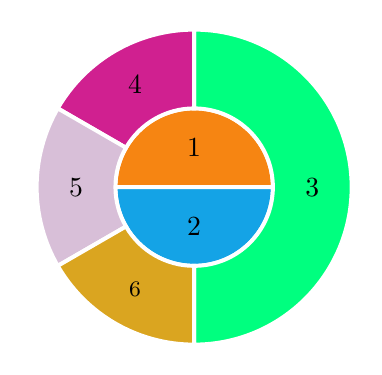
\begin{tikzpicture}[line width=0.05cm]
	\filldraw[fill=BurntOrange,draw=White] (1,0) arc(0:180:1) -- cycle ; \node[color=Black] at (0,0.5) {1} ;
	\filldraw[fill=Cerulean,draw=White] (1,0) arc(0:-180:1) -- cycle ; \node[color=Black] at (0,-0.5) {2} ;
	\filldraw[fill=SpringGreen,draw=White] (90:2) arc(90:-90:2) -- (-90:1) arc(-90:90:1) -- cycle ; \node[color=Black] at (0:1.5) {3} ;
	\filldraw[fill=VioletRed,draw=White] (90:2) arc(90:150:2) -- (150:1) arc(150:90:1) -- cycle ; \node[color=Black] at (120:1.5) {4} ;
	\filldraw[fill=Thistle,draw=White] (150:2) arc(150:210:2) -- (210:1) arc(210:150:1) -- cycle ; \node[color=Black] at (180:1.5) {5} ;
	\filldraw[fill=Goldenrod,draw=White] (210:2) arc(210:270:2) -- (270:1) arc(270:210:1) -- cycle ; \node[color=Black,align=center,font=\fontsize{8pt}{8pt}\selectfont] at (240:1.5) {6} ;
	\end{tikzpicture}
	
	\section{Sample Diagram}
	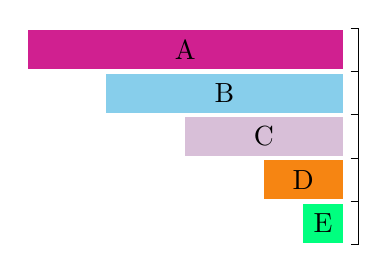
\begin{tikzpicture}[y=1.1cm]
	\draw
	(4.1,4)   -- (4.2,4) -- (4.2,1.5) -- (4.1,1.5)
	(4.1,3.5) -- (4.2,3.5)
	(4.1,3)   -- (4.2,3)
	(4.1,2.5) -- (4.2,2.5)
	(4.1,2) -- (4.2,2) ;
	\fill[color=VioletRed] (0,3.975) rectangle (4,3.525) node[midway,color=Black]{A} ;
	\fill[color=SkyBlue] (1,3.475) rectangle (4,3.025) node[midway,color=Black]{B} ;
	\fill[color=Thistle] (2,2.975) rectangle (4,2.525) node[midway,color=Black]{C} ;
	\fill[color=BurntOrange] (3,2.475) rectangle (4,2.025) node[midway,color=Black]{D} ;
	\fill[color=SpringGreen] (3.5,1.975) rectangle (4,1.525) node[midway,color=Black]{E} ;
	\end{tikzpicture}
	
	\section{Sample Diagram}
	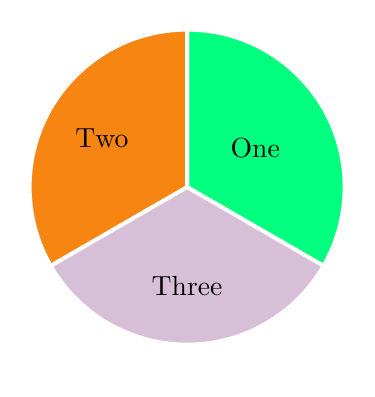
\begin{tikzpicture}[line width=0.05cm]
	\filldraw[fill=SpringGreen,draw=White] (0,0) -- (90:2) arc(90:-30:2) -- cycle ; \node[color=Black] at (30:1) {One} ;
	\filldraw[fill=BurntOrange,draw=White] (0,0) -- (90:2) arc(90:210:2) -- cycle ; \node[color=Black] at (150:1.25) {Two} ;
	\filldraw[fill=Thistle,draw=White] (0,0) -- (210:2) arc(210:330:2) -- cycle ; \node[color=Black,align=center,font=\fontsize{10pt}{10pt}\selectfont] at (270:1.25) {Three} ;
	\end{tikzpicture}
\end{side}
\begin{main}
	\section{Skills}
	
	\begin{bullets}
		\item Aenean vehicula dui sit amet dui sodales porttitor.
		\item Etiam eu lacus aliquet, fermentum augue eget, lobortis ante.
		\item Pellentesque id urna efficitur, finibus ipsum ut, accumsan ante.
		\item Suspendisse sed turpis sit amet ligula lacinia sagittis.
	\end{bullets}
	
	\section{Experience}
	
	\entry{\href{http://anycorp.com}{AnyCorp}}{Web Developer}{2011--2014}
	\begin{bullets}
		\item Sed eget nunc at metus interdum sollicitudin vitae ac augue.
		\item Sed nec augue ultrices, sagittis sapien eu, dapibus diam.
		\item Quisque iaculis ante ac erat placerat vestibulum.
		\item Duis lacinia sapien a vehicula congue
	\end{bullets}
	
	\entry{\href{http://megacorp.com}{MegaCorp}}{Mobile Web Designer}{2008--2011}
	\begin{bullets}
		\item Duis cursus tortor a ipsum volutpat consectetur.
		\item Fusce non metus dictum, egestas dolor a, vehicula mi.
		\item Donec et est accumsan, fermentum elit sed, imperdiet risus.
	\end{bullets}
	
	
	\section{Interests}
	
	\entry{Tea Club}{Executive}{2012--Present}
	\begin{bullets}
		\item Suspendisse vel ex viverra, commodo velit vitae, maximus mi.
	\end{bullets}
	
	\entry{}{Acoustic Guitar}{2004--Present}
	\begin{bullets}
		\item Pellentesque tempus nulla nec diam vulputate luctus.
	\end{bullets}
	
	\section{Achievements}
	
	\begin{bullets}
		\item Nam tempus lorem at metus posuere hendrerit.
		\item Quisque vel nisi quis lacus semper laoreet vel feugiat sapien.
		\item Aliquam pharetra magna sit amet massa porttitor vestibulum.
		\item Cras vitae sem vitae tortor efficitur consectetur.
		\item Quisque ultricies enim non arcu euismod tempor.
		\item Vestibulum varius ex eu accumsan malesuada.
	\end{bullets}
	
	\section{Education}
	
	\entry{Engineering}{University of Waterloo}{2014--2019}
	
\end{main}
\end{document}
